\documentclass[11pt,a4paper]{article}

% ---------- Packages ----------
\usepackage[utf8]{inputenc}
\usepackage[T1]{fontenc}
\usepackage[english]{babel}
\usepackage{lmodern}
\usepackage[a4paper,margin=2.4cm]{geometry}
\usepackage{graphicx}
\usepackage{xcolor}
\usepackage{amsmath}
\usepackage{amssymb}
\usepackage{hyperref}
\usepackage{booktabs}
\usepackage{fancyhdr}
\usepackage{tikz}
\usetikzlibrary{arrows.meta,positioning}

% ---------- Colors ----------
\definecolor{btcgreen}{HTML}{22C55E}
\definecolor{btcgreensoft}{HTML}{86EFAC}
\definecolor{btcdark}{HTML}{0B0F0C}
\definecolor{btcgray}{HTML}{6B7280}
\definecolor{btclight}{HTML}{D1D5DB}

% ---------- Hyperref ----------
\hypersetup{
    colorlinks=true,
    linkcolor=btcgreen,
    urlcolor=btcgreen,
    citecolor=btcgreen,
    pdftitle={CryptoChain Analyzer Dashboard - Final Report},
    pdfauthor={Maria Munoz Nadales}
}

% ---------- Section style ----------
\makeatletter
\renewcommand{\section}{\@startsection{section}{1}{0pt}%
  {2.2ex plus 1ex minus .2ex}{1.0ex plus .2ex}%
  {\color{btcgreen}\large\bfseries\sffamily}}
\renewcommand{\subsection}{\@startsection{subsection}{2}{0pt}%
  {1.6ex plus 1ex minus .2ex}{0.6ex plus .2ex}%
  {\color{btcgreensoft!60!black}\normalsize\bfseries\sffamily}}
\makeatother

% ---------- Header / footer ----------
\pagestyle{fancy}
\fancyhf{}
\renewcommand{\headrulewidth}{0pt}
\fancyfoot[L]{\footnotesize\color{btcgray}CryptoChain Analyzer Dashboard}
\fancyfoot[R]{\footnotesize\color{btcgray}\thepage}

% ============================================================
\begin{document}
\pagenumbering{gobble}

% ---------- COVER PAGE ----------
\begin{titlepage}
\thispagestyle{empty}
\begin{tikzpicture}[remember picture, overlay]
    % Background
    \fill[btcdark] (current page.south west) rectangle (current page.north east);
    % Decorative grid lines
    \foreach \y in {1,2,...,28}{
        \draw[btcgreen, opacity=0.05, line width=0.3pt]
            ([yshift=\y cm]current page.south west) -- ([yshift=\y cm]current page.south east);
    }
    % Top accent bar
    \fill[btcgreen] ([yshift=-3.6cm]current page.north west)
        rectangle ([yshift=-3.65cm]current page.north east);
    % Glow circle
    \fill[btcgreen, opacity=0.10]
        ([xshift=-3cm,yshift=4cm]current page.south east) circle (5cm);
    \fill[btcgreen, opacity=0.06]
        ([xshift=-3cm,yshift=4cm]current page.south east) circle (8cm);
\end{tikzpicture}

\vspace*{2.2cm}
\begin{flushleft}
{\color{btcgreensoft}\sffamily\large CRYPTOGRAPHY \textbar{} FINAL PROJECT REPORT}\\[0.4cm]
{\color{white}\sffamily\fontsize{34}{40}\selectfont\bfseries CryptoChain}\\[0.15cm]
{\color{white}\sffamily\fontsize{34}{40}\selectfont\bfseries Analyzer}\\[0.15cm]
{\color{btcgreen}\sffamily\fontsize{34}{40}\selectfont\bfseries Dashboard}\\[1.2cm]

{\color{btclight}\sffamily\large
A live cryptographic and AI monitor for Bitcoin, Ethereum\\
and Solana network health.}
\end{flushleft}

\vfill

\begin{tikzpicture}[remember picture, overlay]
    \draw[btcgreen, line width=0.8pt]
        ([xshift=2.4cm,yshift=4.6cm]current page.south west) --
        ([xshift=18.6cm,yshift=4.6cm]current page.south west);
\end{tikzpicture}

\vspace{0.8cm}
\begin{flushleft}
\renewcommand{\arraystretch}{1.45}
{\color{btcgray}\sffamily\footnotesize
\begin{tabular}{@{}p{4cm}p{11cm}@{}}
{\color{btcgreensoft}AUTHOR}      & {\color{white}\large Mar\'ia Mu\~noz Nadales} \\
{\color{btcgreensoft}COURSE}      & {\color{white}Cryptography} \\
{\color{btcgreensoft}DELIVERABLE} & {\color{white}Final Report -- Project Documentation} \\
{\color{btcgreensoft}DATE}        & {\color{white}May 2026} \\
\end{tabular}}
\end{flushleft}

\vspace{0.6cm}
\end{titlepage}

% ---------- BODY ----------
\pagenumbering{arabic}

\section{Project Overview}

\emph{CryptoChain Analyzer Dashboard} is a Streamlit application that monitors
three live networks: \textbf{Bitcoin}, \textbf{Ethereum} and \textbf{Solana}.
The interface keeps the same M1--M8 structure for every asset, but adapts the
meaning of each metric to the protocol being inspected. Bitcoin is used for
classic Proof of Work and double-SHA-256; Ethereum focuses on EIP-1559 gas
economics and proof-of-stake security assumptions; Solana focuses on slot
finality, blockhash continuity and throughput stability.

\begin{center}
\small
\renewcommand{\arraystretch}{1.18}
\begin{tabular}{@{}p{2.0cm}p{3.9cm}p{3.9cm}p{3.9cm}@{}}
\toprule
\textbf{Layer} & \textbf{Bitcoin} & \textbf{Ethereum} & \textbf{Solana} \\
\midrule
State & Difficulty, hash rate, block time & Base fee, gas used, block time & Slot, TPS, skip rate \\
Mechanism & 80-byte header, nonce, target & Parent hash, gas target, next base fee & Blockhash, parent slot, finalized status \\
Evolution & Difficulty retargeting & Base-fee trend across recent blocks & TPS and slot-time trend \\
Security & Merkle proof, 51\% attack cost & PoS stake-cost estimate & Skip-rate and finality score \\
\bottomrule
\end{tabular}
\end{center}

\section{Module Structure}

The project follows the mandatory module sequence M1--M4 and extends it with
advanced modules M5--M7. I also added \textbf{M8}, a custom risk-radar module,
because the three chains expose different kinds of risk and a single visual
score makes them easier to compare during a live demo. Some UI labels reuse
the course template names; the table below gives the functional meaning used
in the final multi-chain dashboard.

\begin{center}
\small
\renewcommand{\arraystretch}{1.15}
\begin{tabular}{@{}p{1.25cm}p{3.15cm}p{8.85cm}@{}}
\toprule
\textbf{Mod.} & \textbf{Name} & \textbf{Role in the dashboard} \\
\midrule
M1 & Live state monitor & Shows the current operating state: Bitcoin hash-rate and block time, Ethereum gas load, or Solana TPS and skip rate. \\
M2 & Mechanism analyzer & Opens the protocol object behind the latest state: Bitcoin header fields, Ethereum fee-rule inputs, or Solana parent-slot data. \\
M3 & Evolution history & Plots how the key metric changes over time: difficulty, base fee, or throughput. \\
M4 & AI predictor & Forecasts the next relevant value for each asset using a transparent lightweight model. \\
M5 & Verification module & Recomputes a concrete rule: Bitcoin Merkle inclusion, Ethereum next-base-fee update, or Solana parent-blockhash continuity. \\
M6 & Security score & Translates protocol-specific risk into an interpretable score or curve: 51\% attack risk, PoS capital-at-risk, or finality stability. \\
M7 & Second AI method & Compares linear prediction with exponential smoothing and reports rolling MAE, so the model choice is evaluated. \\
M8 & Custom risk radar & Extra module added by me: a five-factor radar (Security, Finality, Throughput, Fee Health, Stability), useful because BTC, ETH and SOL fail in different ways. \\
\bottomrule
\end{tabular}
\end{center}

\section{Cryptographic Metrics Displayed}

The dashboard displays live evidence that each chain is preserving continuity,
finality and economic security. The metrics are not identical because the
protocols are different, but they answer the same cryptographic question: what
makes the current state hard to rewrite or falsify?

\subsection{Bitcoin: Proof of Work}
For Bitcoin, M2 fetches the raw 80-byte block header and recomputes
the double-SHA-256 block hash:
\[
    H=\mathrm{SHA256}\bigl(\mathrm{SHA256}(\text{header})\bigr).
\]
The result is reversed to Bitcoin display order. The parsed fields are
\texttt{version}, previous block hash,
\texttt{merkle\_root}, timestamp, compact \texttt{bits} and nonce. The compact
target is expanded as $T=c\cdot2^{8(e-3)}$, and a block is accepted when
$H\leq T$. M1 combines difficulty $D$ with recent block time $\bar{t}$ to
estimate hash rate:
\[
    R=\frac{D\cdot2^{32}}{\bar{t}}.
\]
M5 reconstructs a Merkle proof from transaction IDs. M6 implements Nakamoto's
confirmation-risk model for an attacker with hash-rate fraction $q$ after $z$
confirmations~\cite[\S11]{nakamoto2008}.

\subsection{Ethereum: Gas and PoS Security}
For Ethereum, the dashboard replaces mining difficulty with current block
demand. M1 shows block height, base fee, gas used and block time. M2 displays
the parent hash, gas limit, gas target and the protocol-computed next base
fee. M5 recomputes the EIP-1559 update rule from
\texttt{baseFeePerGas}, \texttt{gasUsed} and \texttt{gasLimit}; if the
computed value matches the RPC value, the fee transition is marked
verified~\cite{eip1559}.
M6 estimates economic security from assumed ETH price, total stake and
slashing/loss percentage, exposing how proof-of-stake safety depends on capital
at risk rather than on hash attempts.

\subsection{Solana: Slot Continuity}
For Solana, the relevant evidence is fast finality and slot-chain consistency.
M1 shows finalized slot, TPS, skip rate and average block time. M2 displays
the current blockhash, previous blockhash, parent slot, transaction count and
confirmation depth. M5 verifies that the current slot's declared previous
blockhash matches the parent slot's blockhash, which checks continuity of the
finalized chain. M6 converts skip rate, confirmation depth and slot-time
deviation into an operational security score. The Solana RPC commitment model
defines \texttt{finalized} as the strongest confirmation state used by the
network~\cite{solana_rpc}.

\section{AI Component}

The chosen AI approach is a \textbf{Predictor}. It forecasts the next relevant
network variable for each asset: Bitcoin difficulty, Ethereum base fee and
Solana TPS. M4 provides the main forecast view, while M7 compares a linear
model with exponential smoothing. The common pipeline is:

\begin{center}
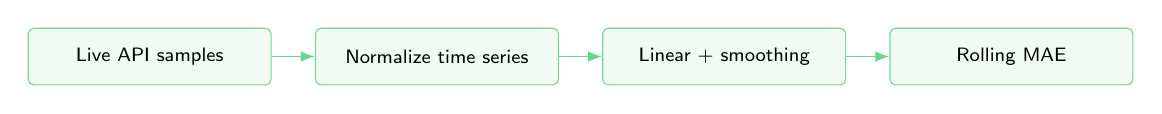
\begin{tikzpicture}[
    node distance=0.55cm,
    box/.style={draw=btcgreen!65, rounded corners=2pt, align=center,
                text width=2.85cm, minimum height=0.72cm,
                fill=btcgreen!6, font=\scriptsize\sffamily},
    arrow/.style={-{Latex[length=1.8mm]}, btcgreen!70, line width=0.65pt}
]
\node[box] (api) {Live API samples};
\node[box, right=of api] (clean) {Normalize time series};
\node[box, right=of clean] (model) {Linear + smoothing};
\node[box, right=of model] (eval) {Rolling MAE};
\draw[arrow] (api) -- (clean);
\draw[arrow] (clean) -- (model);
\draw[arrow] (model) -- (eval);
\end{tikzpicture}
\end{center}

Linear regression was kept because it is transparent: its slope explains
direction and its intercept makes the prediction reproducible. Exponential
smoothing is included because live crypto metrics often move in short bursts;
it gives a second model that reacts more strongly to recent values. Both are
lightweight enough to retrain on every refresh.

\begin{center}
\small
\renewcommand{\arraystretch}{1.18}
\begin{tabular}{@{}p{2.0cm}p{3.4cm}p{3.0cm}p{3.0cm}p{2.0cm}@{}}
\toprule
\textbf{Asset} & \textbf{Predicted metric} & \textbf{Linear MAE} & \textbf{Smoothing MAE} & \textbf{Winner} \\
\midrule
BTC & Difficulty & $3.62{\times}10^{12}$ & $1.16{\times}10^{12}$ & Smoothing \\
ETH & Base fee (gwei) & 0.0192 & 0.0120 & Smoothing \\
SOL & TPS & 100.09 & 77.31 & Smoothing \\
\bottomrule
\end{tabular}
\end{center}

The table was computed on 9 May 2026 with the live dashboard code. It is a
dated evaluation snapshot, so exact MAE values can change when the live APIs
are queried later. Each result
uses a rolling one-step-ahead backtest: train on values before time $t$,
predict $t$, record $|\hat{x}_t-x_t|$, and average the errors. In this run,
exponential smoothing wins for all three assets, so the project reports model
performance instead of assuming that the simpler linear trend is always best.

\section{Conclusion}

The final dashboard is therefore multi-chain, but still cryptographic in
purpose. Bitcoin demonstrates hash-based Proof of Work and Merkle inclusion;
Ethereum demonstrates rule-based fee verification and proof-of-stake economic
security; Solana demonstrates slot finality and blockhash continuity. The AI
component adds an evaluated forecasting layer on top of those metrics, making
the dashboard both explanatory and operational.

% ---------- References ----------
\begin{thebibliography}{9}
\small
\bibitem{nakamoto2008}
S.~Nakamoto, \emph{Bitcoin: A Peer-to-Peer Electronic Cash System}, 2008.\\
\url{https://bitcoin.org/bitcoin.pdf}

\bibitem{eip1559}
V.~Buterin et al., \emph{EIP-1559: Fee market change for ETH 1.0 chain}, 2019.\\
\url{https://eips.ethereum.org/EIPS/eip-1559}

\bibitem{solana_rpc}
Solana Foundation, \emph{Solana RPC Overview}.\\
\url{https://solana.com/docs/rpc}
\end{thebibliography}

\end{document}
